
\section{Progress}
\label{app:progress}

\begin{table}
    \centering
\begin{tabular}{cc}
\hline
    $\boxed{\checkmark}$ & Completed \\
    $\boxed{\times}$ & Not started \\
    $\boxed{+}$ & Started; needs work \\
    $\boxed{-}$ & Remove or scale down \\
    \hline
\end{tabular}    
    \caption{Legend}
    \label{tab:legend}
\end{table}

\begin{table}[]
    \centering


\begin{tabular}{cc|c}


    \hline
    \multicolumn{3}{c}{\textbf{Data}} \\
    \hline
    $\boxed{\checkmark}$ & MNIST & \\ 
    \hline
    \multirow{3}{*}{$\boxed{-}$} & \multirow{3}{*}{Microscopy data} & 
    Requires too much context to explain. \\
    & & It's interesting to see how DeePWAK finds structure in a low quality \\
    & & data set but it's still a low quality data set. \\
    
    \hline
    \multicolumn{3}{c}{\textbf{Outer models}} \\
    \hline
    $\boxed{\checkmark}$ & Encoder & \\
    \hline
    $\boxed{\checkmark}$ & Classifier & \\
    \hline
    $\boxed{\checkmark}$ & Decoder & \\

    \hline
    \multicolumn{3}{c}{\textbf{Inner models}} \\
    \hline
    \multirow{2}{*}{$\boxed{\checkmark}$} & \multirow{2}{*}{SAE} &
    A minimal SAE implementation is available at \\
    & & \url{https://github.com/kewiechecki/SAE} \\
    \hline
    $\boxed{\checkmark}$ & PSAE & see above \\
    \hline
    \multirow{4}{*}{$\boxed{-}$} &  \multirow{4}{*}{DeePWAK} &
    Might be needlessly complicating things. \\
    & & Not straightforward to interpret embed \& unembed. \\
    & & If I want to look at importance of nonlinearity \\
    & & it makes more sense to look at SAE with no $\relu$. \\
    \hline
    \multirow{2}{*}{$\boxed{-}$} & \multirow{2}{*}{DeePWAKBlock} &
    This can be relegated to a separate paper. \\
    & & It doesn't add much for the model I'm working with. \\
    \hline

    \multicolumn{3}{c}{\textbf{Inner model methods}} \\
    \hline
    $\boxed{\checkmark}$ & Encoding & \\
    \hline
    $\boxed{\checkmark}$ & Decoding & \\
    \hline
    $\boxed{\checkmark}$ & Clustering & \\
    \hline
    $\boxed{\checkmark}$ & Cluster centroids & \\
    \hline
    
    \multicolumn{3}{c}{\textbf{Training}} \\
    \hline
    $\boxed{\times}$ & Checkpoints & Save models at different stages of training \\
    \hline
\end{tabular}
    \caption{Model design}
    \label{tab:models}
\end{table}
\begin{table}[]
    \centering
    \begin{tabular}{cc|c}

\hline
$\boxed{\checkmark}$ & Loss &  Figs. \ref{fig:lossouter}, \ref{fig:lossinner} \\
$\boxed{\times}$ & Visualize cluster centroids throughout training &  \\
\hline
\multicolumn{3}{c}{\textbf{Heatmaps}} \\
\hline
$\boxed{+}$ & How to read &  \S \ref{sec:heatmaps} \\
$\boxed{\checkmark}$ & Embeddings &  Fig. \ref{fig:E_MNIST} \\
$\boxed{\checkmark}$ & Clusters &  Fig. \ref{fig:K_MNIST} \\
\hline
\multicolumn{3}{c}{\textbf{Hypergeometric test}} \\
\hline
$\boxed{\times}$ & How to read dot plot &  \\
$\boxed{\checkmark}$ & Dot plot &  Fig. \ref{fig:hyperMNIST} \\
$\boxed{\times}$ & Remove outline scale from dot plot & This is confusing and doesn't add useful information.\\
\hline
    \end{tabular}
    \caption{Data visualization}
    \label{tab:datavis}
\end{table}
\begin{table}[]
    \centering
    \begin{tabular}{cc|c}
    \hline
\multirow{4}{*}{$\boxed{+}$} & \multirow{4}{*}{Git repo} & Code is divided between \\
& & \url{https://github.com/kewiechecki/DeePWAK} and \\
& & \url{https://github.com/kewiechecki/SAE}. \\
& & These need to be unified. \\
\hline
\multicolumn{3}{c}{\textbf{Documentation}} \\
\hline
$\boxed{+}$ & Model documentation & \\
$\boxed{+}$ & Training documentation & \\
$\boxed{\times}$ & Figure documentation & \\
$\boxed{\times}$ & Julia modules & \\
\hline

    \end{tabular}
    \caption{Code distribution}
    \label{tab:docs}
\end{table}
\begin{table}[]
    \centering
    \begin{tabular}{cc|c}
    \hline
$\boxed{\checkmark}$ & \LaTeX template & \\
\hline
$\boxed{\checkmark}$ & Share on Overleaf & 
\hyperlink{https://www.overleaf.com/read/mcvdvdfyfthn#fb5a8e}{view} \\
\hline
\multicolumn{3}{c}{\textbf{Illustrative figures}} \\
\hline
$\boxed{\times}$ & Outer models & \\
\hline
$\boxed{\checkmark}$ & DeePWAK flowchart & Fig. \ref{fig:deepwak} \\
\hline
$\boxed{\times}$ & PWAK example & \\
\hline
$\boxed{+}$ & Diffusion example & Take out DEWAKSS example. Substitute example from actual data. \\
\hline
$\boxed{+}$ & Figure legends & \\
\hline
\multicolumn{3}{c}{\textbf{Algorithms}} \\
\hline
$\boxed{-}$ & noise2self & \\
\hline
$\boxed{-}$ & PWAK & \\
\hline
\multicolumn{3}{c}{\textbf{Supplementary Publications}} \\
\hline
$\boxed{\times}$ & Theoretical foundations & Material cut from \S \ref{sec:2}. Probably post to LessWrong. \\
\hline
\multirow{2}{*}{$\boxed{+}$} & \multirow{2}{*}{DeePWAK} & Split out all microscopy and multihead stuff to \\
& & \url{https://github.com/kewiechecki/DeePWAK} \\
%\url{https://drive.google.com/file/d/1geDArkvUQVOp79dF9knNmO3iP-1BYGOD/view?usp=drive_link}.
\hline
    \end{tabular}
    \caption{Publication}
    \label{tab:pub}
\end{table}

\section{Notation}
\label{app:notation}
We use lowercase Latin characters to denote scalars, boldface lowercase characters to denote vectors, and capital Latin characters to denote matrices.
Subscripts indicate indices.
Because we will mostly be working with matrices in $\mathbb{R}$, we abbreviate $X : \mathbb{R}^{m \times n}$ as $X^{m \times n}$.
We use a circumflex to indicate a reconstruction of an input by a predictor.
Lowercase Greek characters indicate the parameters of a model.
Capital Greek letters indicate parameter spaces.
Function names are in monospace.

\subsection{Layer function notation}
$\fn^{n \to m}$ indicates a layer with input dimension $n$, output dimension $m$, and activation function $\fn$.

$\Conv^{m \times n \times c \to d}_{\fn}$ indicates a convolutional layer that takes a kernel of size 
$m \times n$ with $c$ channels and applies activation function $\fn$. 
It returns $d$ channels for each layer.

$\ConvT^{d \to m \times n \times c}_{\fn}$ indicates a deconvolution layer that takes an input with $d$ channels and returns a reconstructed $m \times n$ output with $c$ channels.

\section{Model architecture}

\subsection{Outer models}
\label{app:outer}
I trained two outer models (Fig. \ref{fig:outermodel}.
Both used an identical convolutional encoder with a 3 neuron information bottleneck.
I first trained the encoder-classifier pair to force the model to represent more than 3 classifications in the bottleneck activations.
I then trained the decoder to reconstruct the images from the latent representation. 

\begin{figure}
     \begin{subfigure}[b]{0.17\textwidth}
        \begin{tikzpicture}[
    node distance = 5mm and 5mm,
    punkt/.style = {rectangle, draw},
    pil/.style = {black, -stealth},
    font=\small
    ]
  \node[punkt,label=above:$\encoder_{outer}^{28 \times 28 \to 3}$] (conv1) {$\Conv^{7 \times 7 \times 1 \to 3}_{\relu}$} ;
  \node[punkt] [below=of conv1] (conv2) {$\Conv^{7 \times 7 \times 3 \to 6}_{\relu}$} ;
  \node[punkt] [below=of conv2] (conv3) {$\Conv^{7 \times 7 \times 6 \to 9}_{\relu}$} ;
  \node[punkt] [below=of conv3] (conv4) {$\Conv^{2 \times 2 \times 9 \to 12}_{\relu}$} ;
  \node[punkt] [below=of conv4](e1) {$\relu^{12 \to 6}$} ;
  \node[punkt] [below=of e1] (e2) {$\relu^{6 \to 3}$} ;

  \draw[pil]
  (conv1) edge (conv2)
  (conv2) edge (conv3)
  (conv3) edge (conv4)
  (conv4) edge (e1)
  (e1) edge (e2);
  
\end{tikzpicture}
         \caption{}
         \label{fig:outerencoder}
     \end{subfigure}
     \hfill
     \begin{subfigure}[b]{0.17\textwidth}
        \begin{tikzpicture}[
    node distance = 5mm and 5mm,
    punkt/.style = {rectangle, draw},
    pil/.style = {black, -stealth},
    font=\small
    ]
  \node[punkt,label=above:$\classifier^{3 \to 10}$] (c1) {$\relu^{3 \to 5}$} ;
  \node[punkt] [below=of c1] (c2) {$\relu^{5 \to 10}$} ;
  \node[punkt] [below=of c2] (softmax) {$\softmax$} ;

  \draw[pil]
  (c1) edge (c2)
  (c2) edge (softmax);
  
\end{tikzpicture}
         \caption{}
         \label{fig:outerclassifier}
     \end{subfigure}
     \hfill
     \begin{subfigure}[b]{0.17\textwidth}
         \begin{tikzpicture}[
    node distance = 5mm and 5mm,
    punkt/.style = {rectangle, draw},
    pil/.style = {black, -stealth},
    font=\small
    ]
  \node[punkt] (conv1) {$\ConvT^{3 \to 7 \times 7 \times 1}_{\relu}$} ;
  \node[punkt] [above=of conv1] (conv2) {$\ConvT^{6 \to 7 \times 7 \times 3}_{\relu}$} ;
  \node[punkt] [above=of conv2] (conv3) {$\ConvT^{9 \to 7 \times 7 \times 6}_{\relu}$} ;
  \node[punkt] [above=of conv3] (conv4) {$\ConvT^{12 \to 2 \times 2 \times 9}_{\relu}$} ;
  \node[punkt] [above=of conv4](e1) {$\relu^{6 \to 12}$} ;
  \node[punkt, label=above:$\decoder_{outer}^{3 \to 28 \times 28}$] [above=of e1] (e2) {$\relu^{3 \to 6}$} ;

  \draw[pil]
  (e2) edge (e1)
  (e1) edge (conv4)
  (conv4) edge (conv3)
  (conv3) edge (conv2)
  (conv2) edge (conv1);
  
\end{tikzpicture}
         \caption{}
         \label{fig:outerdecoder}
     \end{subfigure}
    \hfill
     \begin{subfigure}[b]{0.17\textwidth}
         \begin{tikzpicture}[
    node distance = 5mm and 5mm,
    punkt/.style = {rectangle, draw},
    pil/.style = {black, -stealth},
    font=\small
    ]
    \node[label=above:input data] (X) {$X^{28 \times 28 \times n}$} ;
    \node[punkt] (encoder) [below=of X] {$\encoder_{outer}^{28 \times 28 \to 3}$} ;
    \node[label=right:embeddings] (E) [below=of encoder] {$E_{outer}^{3 \times n}$} ;
    \node[punkt] (decoder) [below=of E] {$\classifier^{3 \to 10}$} ;
    \node[label=below:soft classifications] (Xhat) [below=of decoder] {$K^{10 \times n}$};

    \draw[pil]
    (X) edge (encoder)
    (encoder) edge (E)
    (E) edge (decoder)
    (decoder) edge (Xhat);

\end{tikzpicture}
         \caption{}
         \label{fig:outerenc_inf}
     \end{subfigure}
    \hfill
     \begin{subfigure}[b]{0.17\textwidth}
         \begin{tikzpicture}[
    node distance = 5mm and 5mm,
    punkt/.style = {rectangle, draw},
    pil/.style = {black, -stealth},
    font=\small
    ]
    \node[label=above:input data] (X) {$X^{28 \times 28 \times n}$} ;
    \node[punkt] (encoder) [below=of X] {$\encoder_{outer}^{28 \times 28 \to 3}$} ;
    \node[] (E) [below=of encoder] {$E_{outer}^{3 \times n}$} ;
    \node[punkt] (decoder) [below=of E] {$\decoder_{outer}^{3 \to 28 \times 28}$} ;
    \node[label=below:reconstructed data] (Xhat) [below=of decoder] {$\hat{X}^{28 \times 28 \times n}$};

    \draw[pil]
    (X) edge (encoder)
    (encoder) edge (E)
    (E) edge (decoder)
    (decoder) edge (Xhat);

\end{tikzpicture}
         \caption{}
         \label{fig:outerenc_inf}
     \end{subfigure}
     \caption{Outer model architecture. (\ref{fig:outerencoder}) Encoder submodule shared by both outer models.
     (\ref{fig:outerclassifier}) Classifier submodule.
     (\ref{fig:outerdecoder}) Decoder submodule.
     (\ref{fig:outerclassifier}) Outer classifier forward pass.
     (\ref{fig:outerenc_inf}) Outer decoder forward pass.
     }
     \label{fig:outermodel}
\end{figure}

\subsection{Inner models}
\label{app:inner}

\subsubsection{SAE}
I trained an SAE with a 27 neuron embedding.
Implementation details can be found at 
\url{https://github.com/kewiechecki/SAE}.

\subsubsection{PSAE}
The partitioned sparse autoencoder (PSAE) was identical to the SAE except for the addition of a 12 neuron classifier.

\subsubsection{DeePWAK}
This architecture was identical to the PSAE except for the addition of a nonlinear decoder layer.
Moreover, training it does not include an \textsf{L1} loss.
Implementation details can be found at 
\url{https://github.com/kewiechecki/DeePWAK}.

\section{Self-supervised denoising}
\label{app:bgd}

\subsection{Denoising the data explains the data}
\label{app:ntos}
For a large class of denoising functions, it is possible to find optimal parameters using only unlabeled noisy data\cite{batson2019noise2self}.
$\ntos$ gives a near-maximally-general optimization target for hyperparameter search.


Let $J \in \mathcal{J}$ be independent partitions of noisy data $X$.
Let $\mathcal{F}(\theta)$ be a family of predictors of $X_J$ with tunable parameters
$\theta \in \Theta$ that depends on its complement $X_{J^C}$

\begin{equation}
  \hat{X}_J=\mathcal{F}(\theta)(X_{J^C})
\end{equation}

In other words, $\mathcal{F}$ predicts each data point $X_J$ from some subset of the data excluding $X_J$. 

  The optimal $\theta$ is given by

\begin{equation}
  \label{eq:ntos}
  \ntos_\theta^{\Theta}[\mathcal{F}(\theta),X] := \argmin_\theta^{\Theta}[\sum_{J}^{\mathcal{J}}\mathbb{E}[X_J-\mathcal{F}(\theta)(X_{J^C})]^2]
\end{equation}

\subsection{Diffusion with weighted affinity kernels}

$\ntos$ is particularly useful for finding optimal parameters for generating a graph\cite{tjarnberg2021}.
(see Appendix \ref{app:DEWAKSS})
The adjacency matrix $G$ of any graph can be treated as a transition matrix (or weighted affinity kernel) by setting the diagonal to 0 and normalizing columns to sum to 1. We call this the \WAK function (Algorithm \ref{alg:WAK}).

For each value in data $X$, an estimate is calculated based on its neighbors in the graph. This can be expressed as matrix multiplication.

\begin{equation}
  \label{eq:WAK}
\hat{X} := \WAK(G)X^\top
\end{equation}


\subsection{Partitioned weighted affinity kernels} 
\label{app:pwak}

Though DEWAKSS uses a $k$-NN graph, any adjacency matrix will do.
A clustering can be expressed as a graph where points within a cluster are completely connected and clusters are disconnected.

Let $K^{k \times n}$ be a matrix representing a clustering of $n$ points into $k$ clusters. Let each column be a 1-hot encoding of a cluster assignment for each point. We can obtain a partition matrix $P \in \mathbb{R}^{n \times n}$ by what we'll call the \textit{partitioned weighted affinity kernel} (\PWAK) function.

\begin{equation}
  \label{eq:PWAK}
  \PWAK(K) := \WAK(K^\top K)
\end{equation}

This lets us define a loss function

\begin{equation}
  \mathcal{L}_{\mathPWAK}(K,X) := \mathbb{E}[\mathPWAK(K)X^\top - X]^2
\end{equation}


\PWAK can be extended to soft cluster assignment, making it possible to learn $K$ via SGD.
We will refer to a model of this sort as a \Partitioner to emphasize that while it returns logits corresponding to classifications, there are no labels on the training data.

There is no accuracy measure separate from the decoder loss.
The partitioner simply tries to find the best $P$ for minimizing loss of the decoded output.

The only hyperparameters are the maximum number of clusters, the neural net architecture, and the training hyperparameters.
Because $PX^\top$ is $\mathcal{J}$-invariant, this classifier will converge on a solution less than the maximum $k$.
Intuitions from transformers may be helpful in visualizing why this works.
Informally, $P$ can be equated to position-independent attention with data points as tokens and the batch size as the context window.
Attentive readers may make a connection between masking the diagonal and BERT.

We can now train a model to classify unlabeled data into an undefined number of clusters with no prior distribution in $\mathcal{O}(n^2)$ time!

\begin{figure}
    \centering
    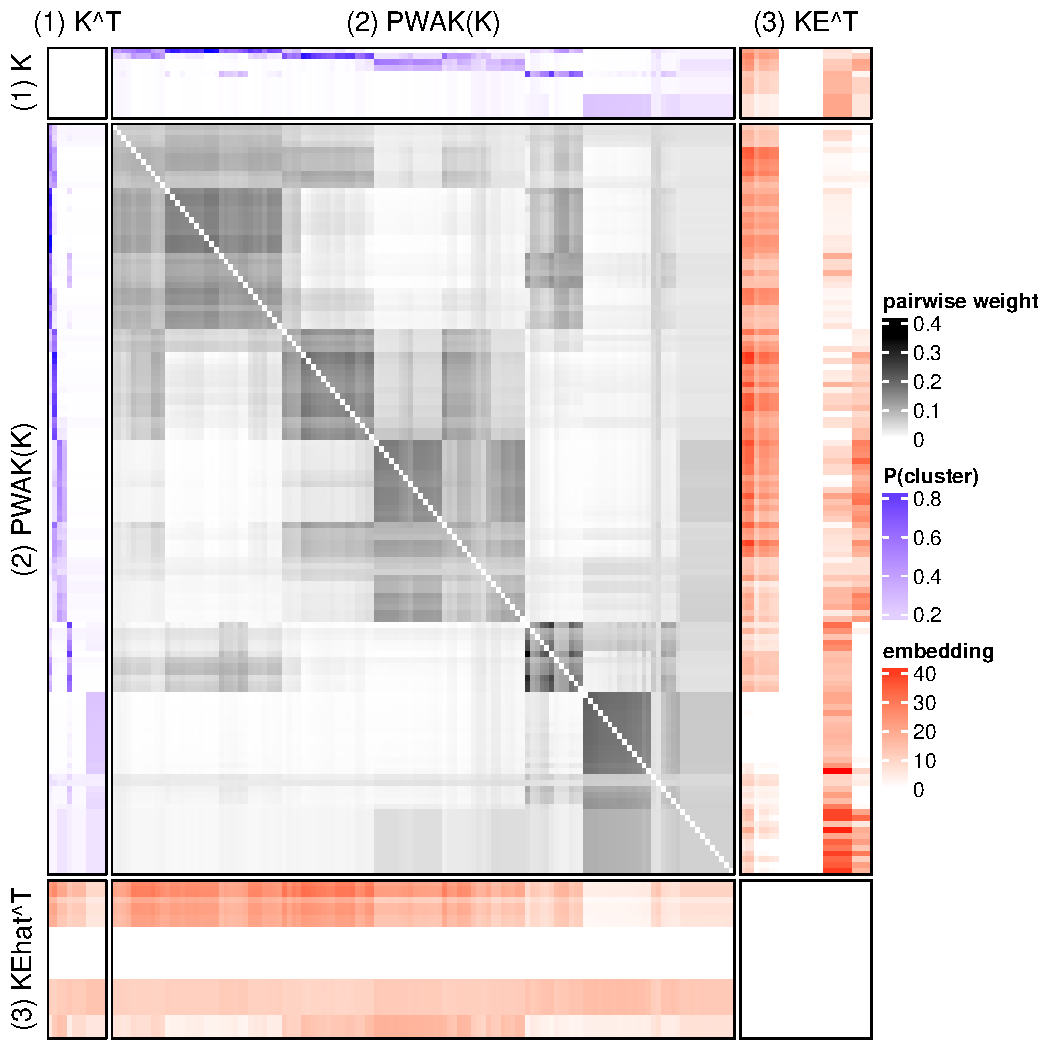
\includegraphics{fig/pwak.pdf}
    \caption{Example of a PSAE forward pass. Indices for subfigures are given as \textsf{(column,row)}.
    \textsf{(1,2)} and \textsf{(2,1)} show the predicted clusters.
    \textsf{(2,2)} is the partition matrix, obtained by applying the \PWAK transformation to the do product of
    \textsf{(1,2)} and \textsf{(2,1)}.
    \textsf{(3,2)} shows the embeddings obtained by the inner encoder.
    \textsf{(2,3)} shows the dot product of \textsf{(2,2)} and \textsf{(3,2)}, which corresponds to the denoised embeddings.
    \textsf{(3,1)} shows the dot product of \textsf{(2,1)} and \textsf{(3,2)}. This corresponds to finding the centroid of
    each cluster.
    \textsf{(1,3)} shows the dot product of \textsf{(1,2)} and \textsf{(2,3)}. This gives the denoised centroids.
    Presenting the data this way suggests an obvious optimization:
    instead of calculating the embeddings for each batch, can we just learn the cluster centroids?
    }
    \label{fig:pwak}
\end{figure}

\section{Bisemanticity in microscopy data}
\label{app:micro}
\secsubhead{
This section is especially disorganized. I was uncertain whether to include any of these results.
I ultimately decided to include a bare minimum to convey my thoughts on the link between 
bisemantic features and latent decision trees\cite{aytekin2022neural}.
}

Most of the theory for this project was originally developed for unsupervised phenotype detection
from microscopy images.
For these data the implementation of the encoder and decoder differed from a canonical SAE,
but the inner model still conformed to the spec in Fig. \ref{fig:deepwak}.
A larger difference was that I used an ensemble method consisting of 5 encoder/classifier heads.
Despite these differences, I think these results complement the MNIST results in a few ways.

\begin{figure}
    \centering
    \begin{tikzpicture}[
    node distance = 5mm and 5mm,
    punkt/.style = {rectangle, draw},
    pil/.style = {black, -stealth},
    font=\small
    ]

  %\node[punkt] (preprocessing) {preprocessing} ;
  \node[] (X) {$X$} ;

  \node[punkt] (h3) [right=of X] {$\mathDeePWAK$} ;
  \node[punkt] (h2) [above=of h3] {$\mathDeePWAK$} ;
  \node[punkt] (h1) [above=of h2] {$\mathDeePWAK$} ;
  \node[punkt] (h4) [below=of h3] {$\mathDeePWAK$} ;
  \node[punkt] (h5) [below=of h4] {$\mathDeePWAK$} ;

  %\node[] (Xhat1) [below=of h1] {$\hat{X}_1$} ;
  %\node[] (Xhat2) [below=of h2] {$\hat{X}_2$} ;
  %\node[] (Xhat3) [below=of h3] {$\hat{X}_3$} ;
  %\node[] (Xhat4) [below=of h4] {$\hat{X}_4$} ;
  %\node[] (Xhat5) [below=of h5] {$\hat{X}_5$} ;

  %\node[punkt] (sum) [right=of h3] {$\sum$} ;
  \node[] (concat) [right=of h3] {$\oplus$} ;
  \node[punkt] (linear) [right=of concat] {$\linear^{5 \times m \to m}$} ;
  \node[] (Xhat) [right=of linear] {$\hat{X}$} ;
  %\node[punkt] (loss) [below=of h5] {MSE} ;
  %\node[] (grad) [right=of loss] {$\nabla$} ;
  %\node[punkt] (update) [right=of grad] {$\mathrm{update!}(\theta,\pi,\phi)$} ;
  
  \draw[pil] %(preprocessing) edge (X)

  (X) edge[bend left=30] (h1)
  (X) edge[bend left=30] (h2)
  (X) edge (h3)
  (X) edge[bend right=30] (h4)
  (X) edge[bend right=30] (h5)

  (h1) edge[bend left=30] (concat)
  (h2) edge[bend left=30] (concat)
  (h3) edge (concat)
  (h4) edge[bend right=30] (concat)
  (h5) edge[bend right=30] (concat)

  (concat) edge (linear)
  (linear) edge (Xhat) ;
  %(sum) edge[bend left=15] (Xhat) ;
  %(Xhat) edge[bend left=15] (loss) 
  %(X) edge[bend right=30] (loss)
  %(loss) edge (grad)
  %(grad) edge (update);
\end{tikzpicture}

  

    \caption{Multihead DeePWAK. Each head is as shown in Fig. \ref{fig:deepwak}.
    The final result is obtained through a linear combination of the outputs 
    of each head.}
    \label{fig:block}
\end{figure}

\begin{enumerate}
    \item It is a much smaller, less well-characterized data set
    \item The information content is nonobvious
    \item It's an independent toy model of feature aggregation: there is lots of redundant information,
    but the relations are nonobvious
    \item Linear methods fail to characterize the features well
\end{enumerate}

I mostly want to draw your attention to \ref{fig:blockE}, which gives a striking example of bisemanticity.
\textsf{Heads2-5} each seem to distinguish a All of the more nuanced discrimination happens in \textsf{Head1}.
This is suggestive that the model may in fact be learning a tree structure to split the data along major features. These major features effectively split experimenter-labeled phenotypes (Fig. \ref{fig:hyper}). 

It splits the data into almost but not quite the maximum number of clusters, indicating our choice of $k$ is close to the latent concept space for (this projection of) the data.
Fascinatingly, the embeddings are even sparser.

\begin{figure}
  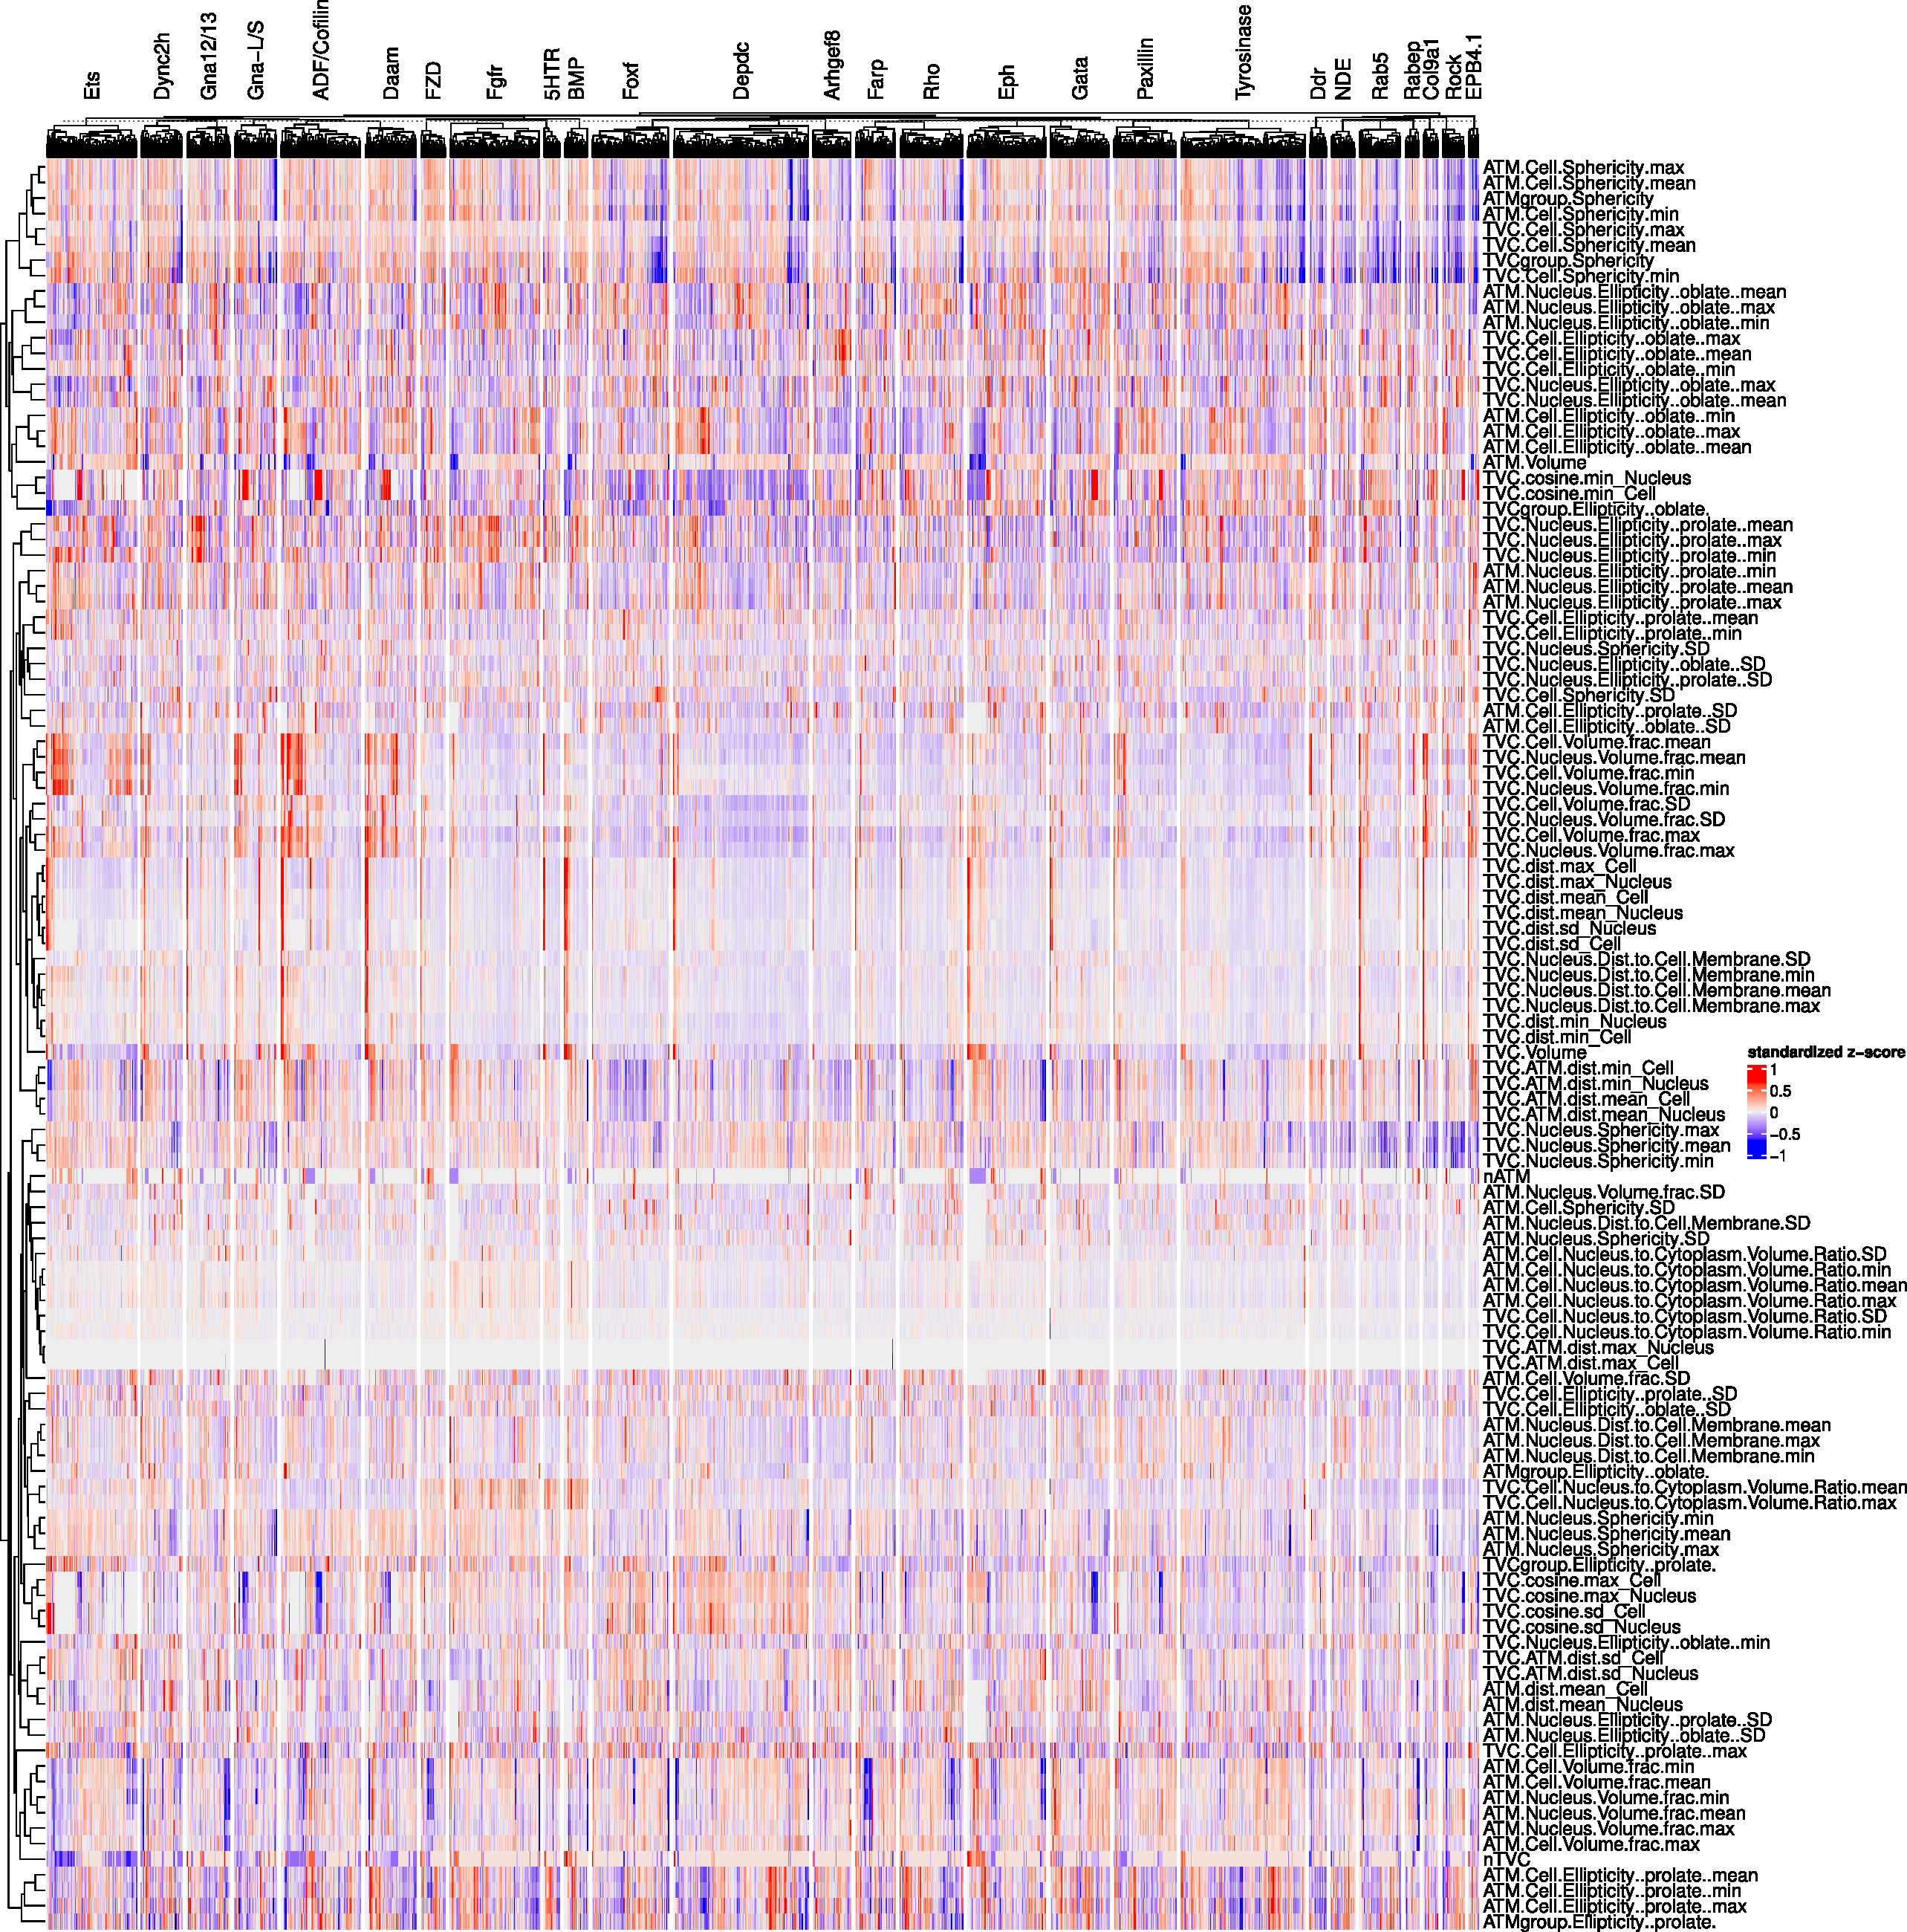
\includegraphics[width=\textwidth]{params.pdf}
    \caption{Preprocessed microscopy data from 1853 embryos.
    I took a very crude approach to preprocessing, 
    extracting 114 ad hoc statistics with no consideration for redundancy or significance.
    The seeming poor quality of this data set hides a surprising amount of structure.
    }
    \label{fig:params}
\end{figure}

\begin{figure}
  %\begin{subfigure}[b]{0.5\textwidth}
  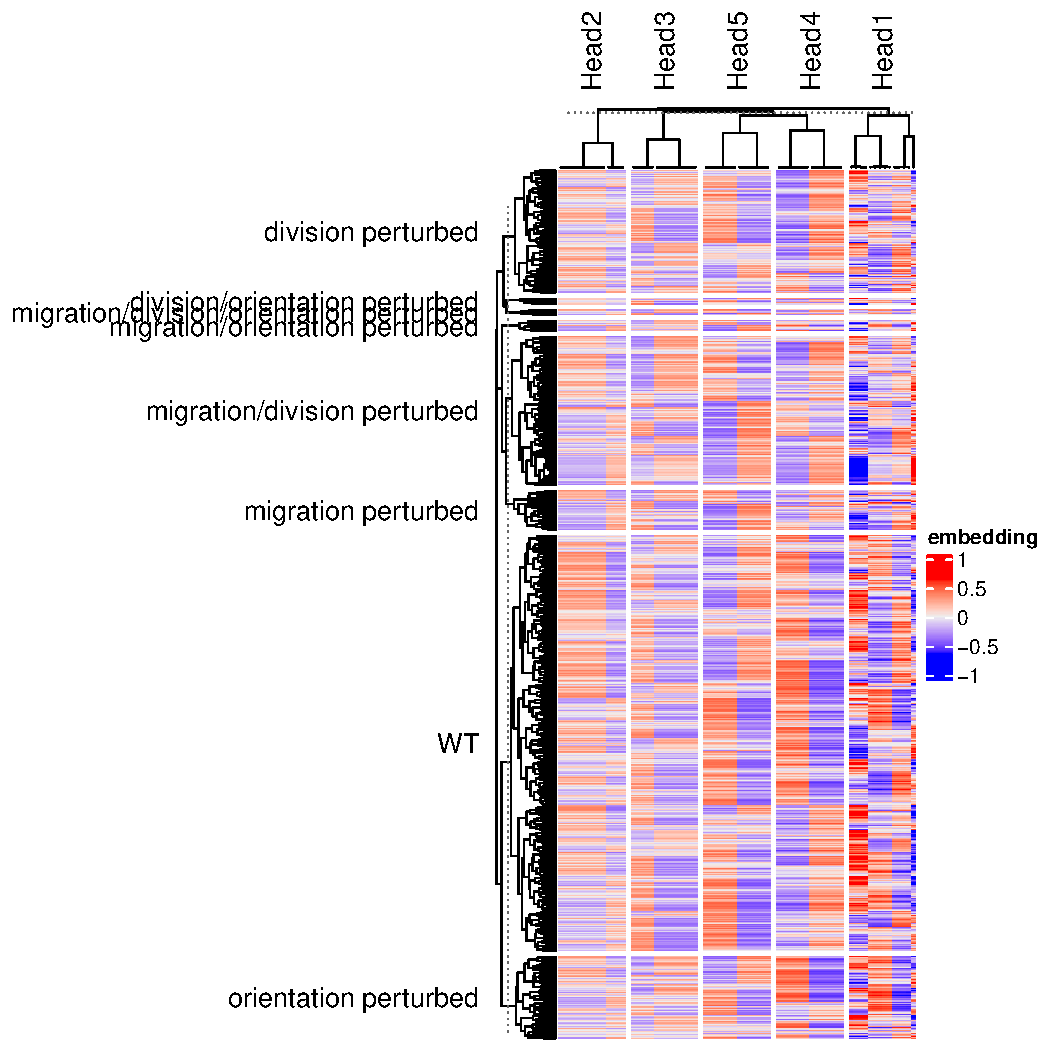
\includegraphics[width=\textwidth]{embeddings.pdf}
    \caption{DeePWAK learns sparse embedding values. 
    Each head actually has 14 embeddings, but for all but \textsf{Head1}, 
    they converge to two embeddings. 
    }
    \label{fig:blockE}
\end{figure}
